\documentclass[a4paper, twoside]{article}
\usepackage[T1]{fontenc} % Font encoding, T1 = it
\usepackage[utf8]{inputenc} % Input encoding - per caratteri particolari
\usepackage[english]{babel} % Lingua principale italiano, con parti in inglese
\usepackage{graphicx} % Per includere immagini esterne

\usepackage{lipsum} % genera testo fittizio
\usepackage[a4paper,top=3cm,bottom=3cm,left=2.5cm,right=2.5cm,footskip=.25in]{geometry} %impaginazione e margini documento
\usepackage[fontsize=11pt]{scrextend} %dimensione font
\usepackage{float}
\usepackage{booktabs}
\usepackage{titlesec}
\usepackage[font=small,skip=0pt]{caption}
\usepackage{wrapfig}
\usepackage[%  
    colorlinks=true,
    pdfborder={0 0 0},
    linkcolor=red
]{hyperref}

\usepackage{enumitem}

\usepackage{fancyvrb} % for "\Verb" macro

\setlength{\textfloatsep}{2pt}     % Space between text and float
\setlength{\intextsep}{2pt}    

\titlespacing{\section}{1pt}{\parskip}{-\parskip}
\titlespacing{\subsection}{1pt}{\parskip}{-\parskip}
\titlespacing{\subsubsection}{1pt}{\parskip}{-\parskip}


\begin{document}
\input{frontespizio}

\section{Introduction}
Our work is about to analyze and extract a perfect clean data for usage of machine learning training. This work is applied to 2 different datasets: cyclists dataset and race dataset. Sequence of action made for elaborate datasets are:

\begin{enumerate}[noitemsep]
    \item Analyze distribution and correlation between features.
    \item Fill missing data and delete useless features for cleaning datasets.
    \item Feature engineering for managing missing values and adding more useful informations.
    \item Applying clustering for analyzing pattern inside the datasets.
    \item Prepare a dataset for machine learning and train a set of models to it.
\end{enumerate}

\section{Data understanding}

Data understanding phase was applied for have a general view about: distributions value, missing value distributions, semantically checking of values for each feature. From this analyis it was taked decision about data transformation and feature engineering.

\subsection{Feature distributions}

After a discrete analysis, it is possible to see that almost all the features have a gaussian distributions (except for points, uci\_points and profile). This allow to use gaussian distributions when sampling can be necessary. In this analysis, features like nationality, team\_cyclists etc. are not analyzed because string values are not relevant (also because is difficult to analyze distribution to a non numerical domain).

\subsection{Correct values check}
The objective of this analysis is to ensure that the dataset is free of potential errors, such as invalid or incorrectly formatted entries, duplicates, and discrepancies that could hinder the analysis. Validating these aspects is crucial for data integrity and consistency before proceeding to complex tasks, such as feature engineering or machine learning.
.

\textbf{Observations}

Analysis of the Cyclists and Race datasets reveals key findings:
\begin{itemize}[noitemsep]
    \item Some cyclists only appear in one dataset (for example, in \texttt{Race} but not in \texttt{Cyclists}), requiring updates to ensure that all cyclists in one dataset are also in the other.
    \item Three main issues are identified in the \texttt{Race} dataset:
    \begin{enumerate}[noitemsep]
        \item \textbf{Points Duplication Issue}: The \texttt{points} and \texttt{uci\_points} columns contained identical values across all cyclists within each race. These values appeared to be copied from the first-place finisher's point allocation.
        \item \textbf{Position Recording Issue}: Disqualified cyclists retained their original positions in the dataset. Subsequent riders were incorrectly shifted down one position. For example, if a cyclist in 15th place was disqualified, the replacement rider was incorrectly listed in 16th place.
        \item \textbf{Negative Deltas}: The \texttt{delta} column contained negative values for some cyclists. These negatives arose from different representations where the first rider's time was used as a reference point, and all other riders' times were subtracted from it. For example, if the first rider's time was \texttt{0:46:18}, subsequent riders had negative deltas like \texttt{-44:05}, \texttt{-44:02}, etc. We assumed that the correct delta should represent the difference between the first rider's time and subsequent riders' times.
    \end{enumerate}
\end{itemize}

\textbf{Proposed Solution}

To resolve these issues, we scraped \texttt{ProCyclingStats} for the correct data. 

By scraping the data, we observed the following:
\begin{itemize}[noitemsep]
    \item Some cyclists were present only in the \texttt{Cyclists} dataset, which is normal since disqualified cyclists were excluded from our updated dataset.
    \item Some cyclists were present only in the updated \texttt{Race} dataset, which is not normal. To address this, we enhanced the scraping process to look for the missing cyclists in the \texttt{Cyclists} dataset and add them to the updated \texttt{Race} dataset. The missing cyclists' information was obtained from the same source.
\end{itemize}

\subsection{Missing values}

An analysis was done on the datasets to better understand the distribution of missing values in the datasets. This analysis served to better understand which applications need to be made in the data transformation phase, understanding how to fill the missing data and whether a merging phase between the datasets is necessary to fill some columns.

In the cyclist dataset, as can be seen from the figure  ~\ref{fig:missing-value-cyclists-dataset}, we can see that:
\begin{itemize}[noitemsep]

    \item \textbf{birth\_year} = the column has 21 missing values and will be filled, as it is relevant as a characteristic.

    \item \textbf{weight} / \textbf{height} = There are 2 columns with 3241 and 3176 missing values respectively and they will be filled.

    \item \textbf{Nationality} = Even if it is not a relevant feature, it will be filled by searching for the only missing value on the internet.

\end{itemize}
In the race dataset, as can be seen from the figure ~\ref{fig:missing-value-race-dataset}, we can see that:

\begin{itemize}[noitemsep]

    \item \textbf{uci\_points} = the column has 346245 missing values, so a transformation is necessary, as it contains an important alternative score for the races (international cycling union score).

    \item \textbf{climb\_total} = the column has 153766 missing values and a transformation is necessary, as the total distance of the route is relevant.

    \item \textbf{profile} = the column has 155351 missing values, and contains the difficulty of each race, therefore an important feature to fill.

    \item \textbf{average\_temperature} = the column contains more missing values than all: 567440 missing values but it will not be filled, because it is not correlated to other characteristics and it is not safe to sample values from a distribution, as the temperature is an influencing factor of the race, being that it influences the athlete's body during the race.

    \item \textbf{cyclist\_team} = the column contains 2457 missing values but will not be filled, as the team name is not relevant.

    \item \textbf{delta} = the column contains 50259 missing values, and the difference between the first comer is a feature with its impact of importance.

\end{itemize}

\subsection{Correlation between features}
The subsequent analysis of column relationships will investigate various elements of the riders' performance, identify traits for data imputation and explore potential correlations that could inform predictive modeling.
\subsubsection{Correlation Matrix}
We begin the feature correlation exploration by examining the correlation matrix (Figure \ref{fig:correlation-matrix}), which includes all the numerical features from both datasets combined.
\begin{figure}[ht]
    \centering
    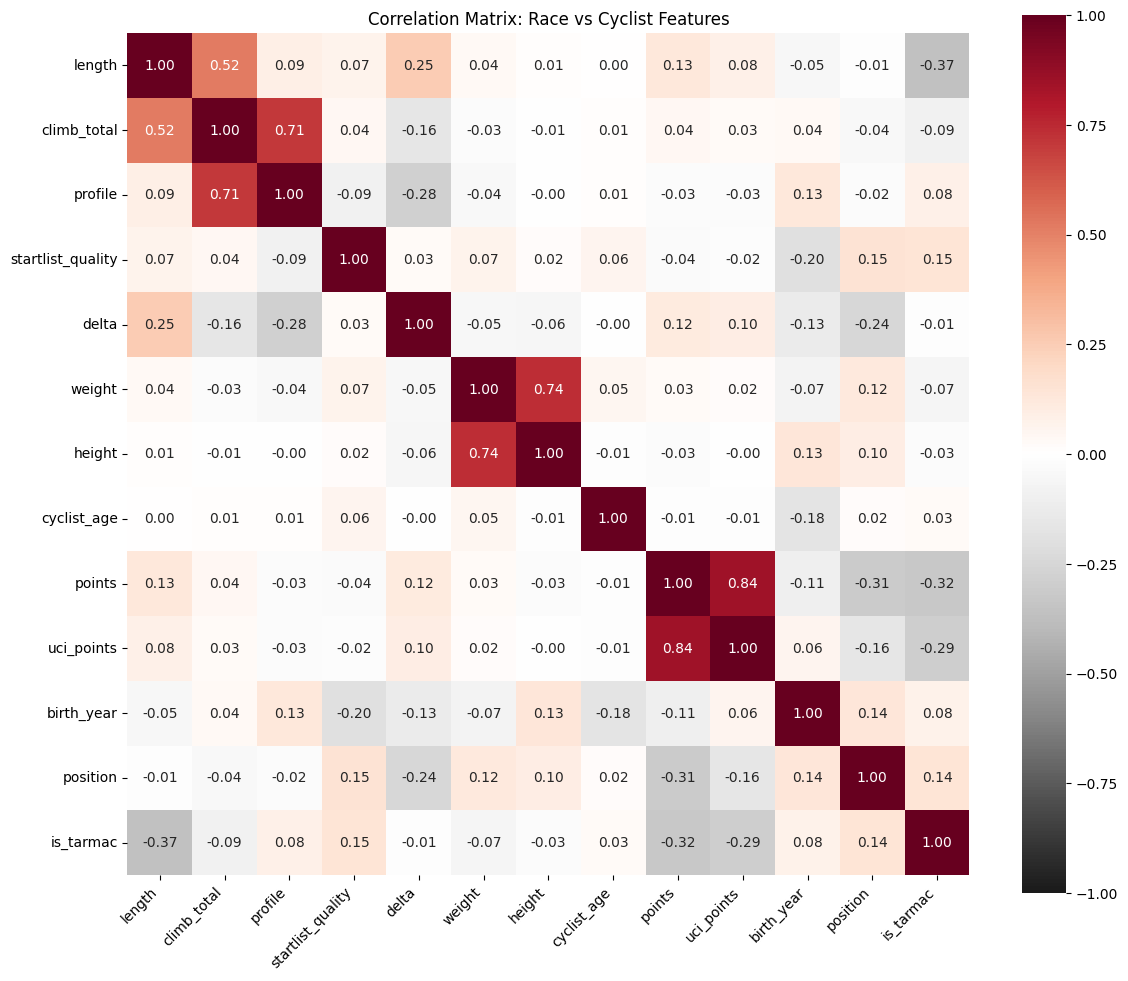
\includegraphics[width=0.75\textwidth]{assets/correlation_matrix.png}
    \caption{Correlation matrix between all relevant features.}
    \label{fig:correlation-matrix}
\end{figure}

We can observe strong positive correlations: \texttt{height} vs.\ \texttt{weight} (0.74), \texttt{climb\_total} vs.\ \texttt{profile} (0.71), and \texttt{points} vs.\ \texttt{uci\_points} (0.84). We also find a notable positive correlation between \texttt{climb\_total} and \texttt{length} (0.52) and a weaker one for \texttt{delta} and \texttt{length} (0.25).

On the negative side, \texttt{length} is weakly correlated with \texttt{is\_tarmac} (0.36), suggesting that longer races are less likely to be primarily on tarmac. \texttt{Points} also shows a negative correlation with \texttt{is\_tarmac} (0.32), implying that higher-point races often include varied terrain. Other negative correlations include \texttt{points} vs.\ \texttt{position} (0.31) and \texttt{profile} vs.\ \texttt{delta} (0.28), where the latter suggests that more challenging profiles may result in smaller time gaps, possibly due to tighter rider grouping.
\subsubsection{Points, Age, Temperature and Career Span}
Even though the number of available \texttt{average\_temperature} samples is limited, it is informative to compare how age groups perform across different temperature ranges.

\begin{figure}[ht]
    \centering
    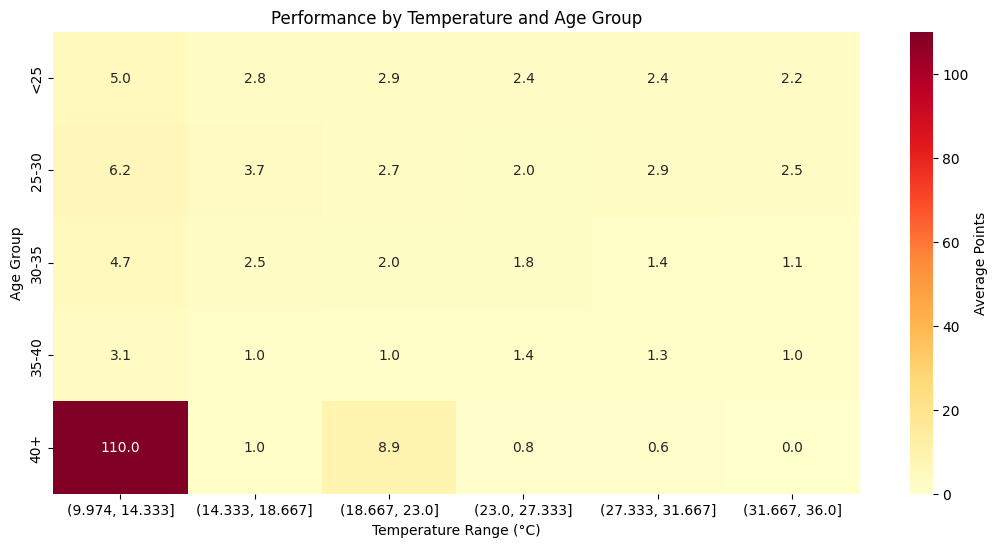
\includegraphics[width=0.85\textwidth]{assets/perf_age_group.png}   
    \caption{Average points by age group, temperature range and age distribution.}
    \label{fig:temperature-age}
\end{figure}

As shown in Figure \ref{fig:temperature-age} (first plot), the 40+ group exhibits high average points (110.0) within the (9.9--14.3) temperature range, and 8.9 points within the (18.6--110.0) range. However, this group has a very small sample size (Figure \ref{fig:temperature-age} second plot), partly because riders often retire before reaching 40. Consequently, the limited data for this group may skew the average.
 \\
Although there is no observed correlation between cyclist age and points, it remains compelling to examine how age influenced rider performance and cyclists' career length.
Therefore next, we examine how age correlates with riders' performance and career duration. Figure~\ref{fig:w-h-p-corr}, first plot, shows a bell-shaped distribution, indicating that for most cyclists, age has a limited impact on performance. Some riders experience a decline, while others improve as they age.
The age-performance correlation plot highlights outliers at the tail of the distribution. The strong negative correlation suggests some cyclists excelled early in their careers, but then experienced a marked decline. Conversely, others started with weaker performances and improved significantly over time.
The second right-skewed distribution, Figure~\ref{fig:w-h-p-corr} second plot, likely reflects the sport's high physical demands: many riders competed for no more than three years, and relatively few pursued extended careers.
\subsubsection{Physical Attributes, Performance and Race Profile}
Finally, we explore how physical attributes may affect a rider's final position across different race profiles. We also identify which personal features dominate in each profile.
\begin{figure}[ht]
    \centering
    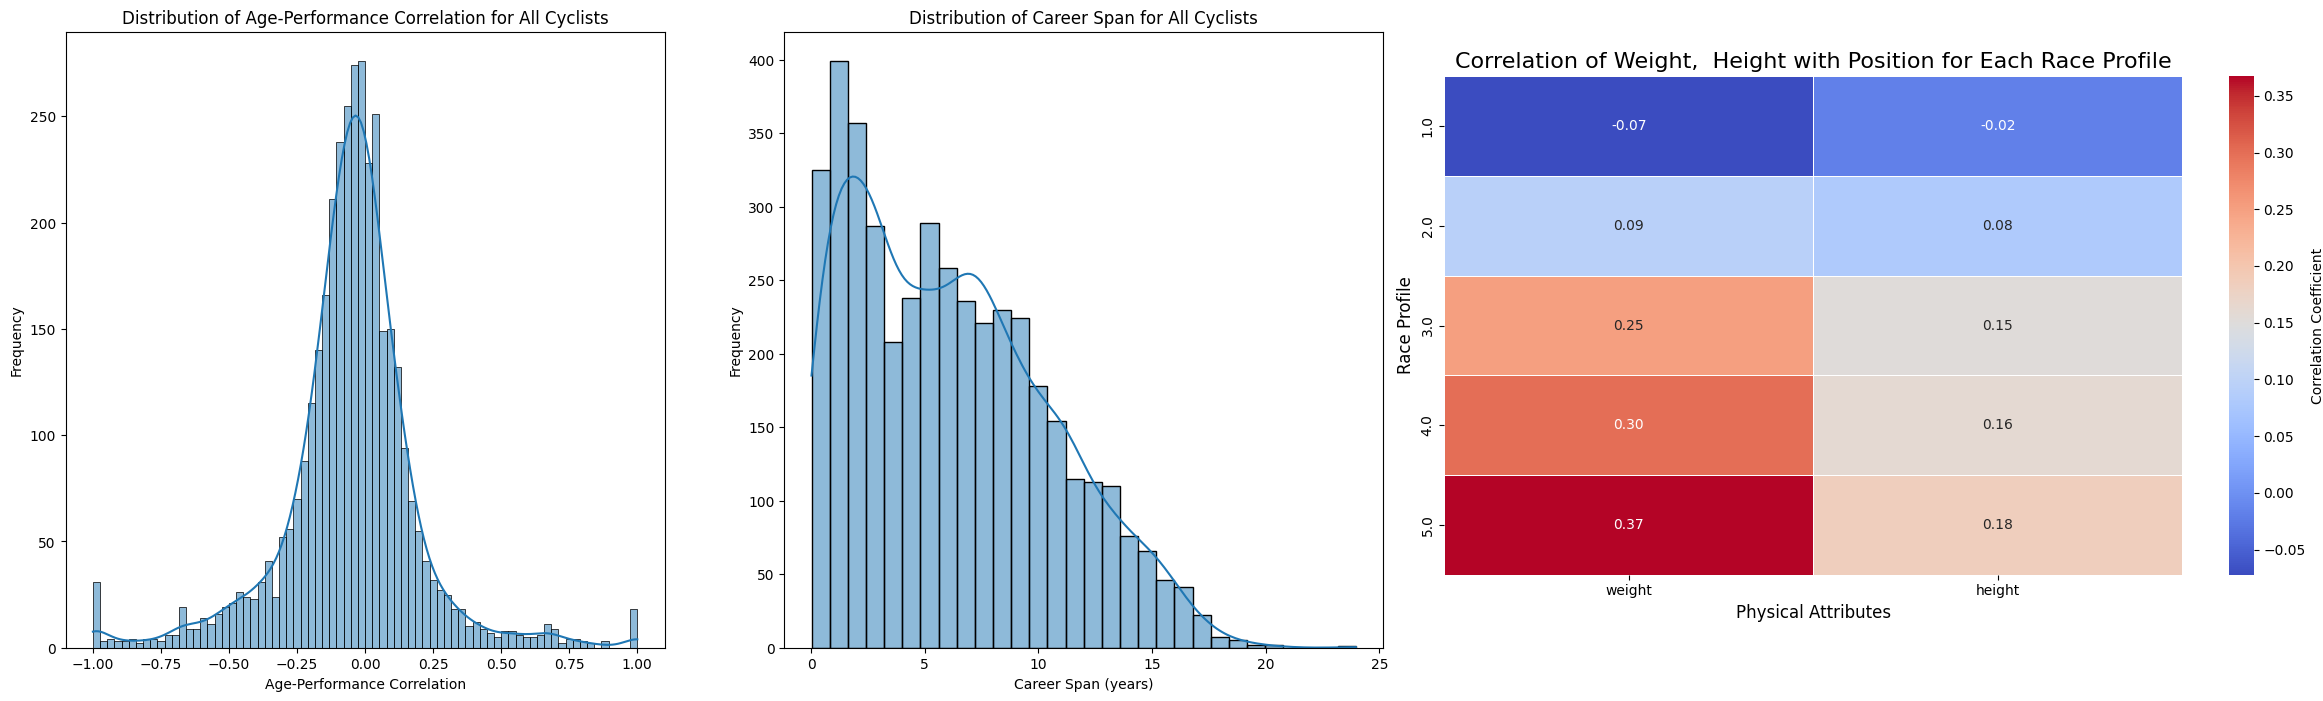
\includegraphics[width=1.0\textwidth]{assets/w_h_p_corr.png}
    \caption{Mixture of plots}
    \label{fig:w-h-p-corr}
\end{figure}
The Figure~\ref{fig:w-h-p-corr}, third plot, indicates that as climb difficulty increases, \texttt{weight} and \texttt{height} become more critical in determining a rider's final position. Notably, \texttt{weight} strongly influences outcomes in high mountain races, compared to \texttt{height}.
\\
For each race profile, we highlight the top 10 riders for that profile alongside their five key attributes, illustrating the qualities required to stand out in a specific race type.
In the Figure~\ref{fig:top_perf_profile}, BMI stands for Body Mass Index. The \texttt{experience} is calculated using the formula: 
\verb+(race_date - career_start).dt.days / 365.25+.
\\
Here, \verb|race_date| is the date of the race, and \verb|career_start| is the date of the cyclist's first race.
\begin{figure}[ht]
    \centering
    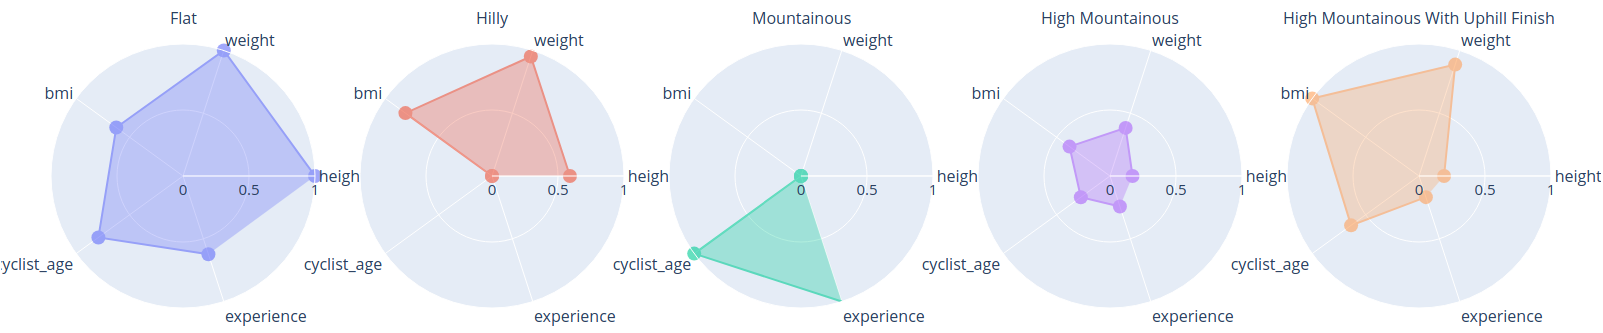
\includegraphics[width=0.85\textwidth]{assets/top_perf_profile.png}
    \caption{Mean physical features of 10 best riders per profile}
    \label{fig:top_perf_profile}
\end{figure}
Heavier, taller, and more experienced mid-career riders tend to excel on flat profiles. Heavier, average-height, young cyclists excel in hilly race profiles. Heavier, shorter, and experienced adult cyclists stand out in mountainous race profiles. However, in high mountainous terrain, slightly heavier, taller, less young, and less experienced riders perform well. Finally, in high mountainous races with an uphill finish, the best cyclists are on average heavier, shorter, middle-aged, and less experienced
\subsubsection{Motivation}
We focused on these analyses in the report because they highlight key aspects of professional cycling performance that can help better understand the factors influencing a cyclist's career. For example, the career span distribution shows that, on average, riders do not remain active in professional cycling for long. Additionally, the bell-shaped distribution suggests that riders must train consistently to stay competitive. The temperature analysis is compelling because it shows how different age groups perform in various conditions, and on average, cyclists tend to achieve better results in lower temperatures.
The physical attributes analysis is informative because it reveals how a rider's weight and height influence their performance across different race profiles. Finally, the top 10 riders' physical attributes for each profile provide insights into the qualities required to excel in different race types. \\
We believe that these analyses can help us in subsequent tasks, such as feature engineering and model building, by providing a better understanding of the relationships between different features and how they influence a cyclist's final position. By identifying the key attributes that contribute to a rider's success, we can create more accurate models.

\section{Data transformation}

This is a crucial phase because in this part, every missing value was filled using knoweldge discovered by data understanding (distributions and correlations). Every column with at least one missing value were filled with appropriate technique (sampling, derived by other column(s), missing values searched manually on internet etc.).

\subsection{Fill missing data}

According to results coming from analyzing missing data distributions from data understanding, it was necessary to fill missing data values. First of all, the semantic and statistical correlation between the columns with missing data was analyzed, in fact some values were derived from others, and other values were filled by searching for them on the Internet.

For \textbf{cyclist dataset}, filling data was in:

\begin{itemize}[noitemsep]

    \item \textbf{Nationality} column = nationality column had only 1 missing values, so it was filled manually (searched by Google).

    \item \textbf{birth year} column = birth year column had few missing values (13), so they were filled manually (searched by Google).

    \item \textbf{weight} and \textbf{height} columns = It was find out that these 2 columns are correlated each other, so it was used 2 linear regression, one linear regression trained with weight values for predict height value for fill height values (with weight aviable) and other linear regression for viceversa. For training was used of course all raw where both weight and height was not missing). For filling values where both weight and height was missing, it was used a multivariate gaussian distribution and values where filled with sampling from this distribution.

\end{itemize}

For \textbf{race dataset}, filling data was in:

\begin{itemize}[noitemsep]

    \item \textbf{average temperature} column = Considering that was so much missing values (557121), there was not any correlations with other features and was useless (after a discussion), it was decided do delete the feature.

    \item \textbf{cyclist age} column = This column was derived from birth year column (from cyclist dataset) and date column (from race dataset). For each row, cyclist age was calculated doing difference between date year of race and birth year of cyclist. This operation was applied also for substitute aviable values, for be sure that age values was correct.

\end{itemize}
\subsubsection{Imputation of \texttt{uci\_points}, \texttt{climb\_total}, \texttt{profile} and \texttt{delta} null values}
We imputed missing values with special filling, since these features are crucial for subsequent analysis and modeling tasks. Consequently, basic imputation methods alone would be insufficient to maintain the foundational data distributions. As stated earlier, some are related linearly, while others are not. The table \ref{tab:imputation-comparison} indicates that adopting more sophisticated imputation techniques was beneficial. It helped to have small fraction of absent and some columns correlations (e.g., \texttt{uci\_points} with \texttt{points}).
\\ The main benefit of this approach is the preservation of the dataset's original size, hence more samplers for classification/prediction tasks. The disadvantages are that the imputed values must align with existing feature patterns to maintain data integrity, which can be guaranteed in some cases  only with advance strategies.
\subsubsection{Methodology Overview}
We tested three main approaches to impute the missing data:
\begin{itemize}[noitemsep]
    \item \textbf{Regression method}: 
    It trains 10 regressors with 5-fold cross-validation, compares the average results, and selects the best model by RMSE (Root Mean Square Error) metric. \\ 
    We used random search to determine well performing hyperparameters, which remained fixed in subsequent experiments to reduce computation time. The hyperparameters starting ranges were set to typical values found in the literature.
    \item \textbf{Densities method}:
    It clusters data by shared characteristics, identifies the best-fitting statistical distribution from one of ten possible ones, for each segment (cluster), and uses the identified best-fit distribution to predict missing target values  within the respective cluster.
    \item \textbf{Clustering method}:
    It uses scikit-learn’s \texttt{KNNImputer} to fill missing values by locating their nearest neighbors with a KNN-based approach and imputing with the neighbors’ mean.
\end{itemize}

\subsubsection{Set up}
The results analyses will focus only on \texttt{climb\_total} imputation, but the same methodology was applied to the other features, which gave similar outcomes.\\
The numerical features were scaled using \texttt{MinMaxScaler(feature\_range=(-1, 1))}, and the categorical data were encoded as positive integers. \\
To evaluate with supervised metrics, we excluded empty value rows where was necessary. We split the dataset 80-20 into training and test sets.
The training set was used for model fitting and validation, while the test set evaluated performance on unseen data.

\subsubsection{Motivation}
These three methods address relationships among variables, data distribution, and sample proximity. Regression imputation uses feature relationships, density-based imputation preserves variability, and KNN captures local patterns.
Using the right evaluation strategy and metrics for the above methods, we identified suitable values to fill missing data.
\\
We selected these methods because they offer flexibility, they balance complexity, and they can capture a wide range of data patterns.
\subsubsection{Multiple Regressor Approach}
We decided to use these regressors: \texttt{Random Forest}, \texttt{Gradient Boosting}, \texttt{XGBoost}, \texttt{Huber}, \texttt{Linear Regression}, \texttt{Ridge}, \texttt{Lasso}, \texttt{KNeighborsRegressor}, \\ \texttt{HistGradientBoostingRegressor} and \texttt{VotingRegressor} because they cover a wide spectrum of modeling approaches and have complementary strengths:
\begin{itemize}[noitemsep]
    \item Traditional linear methods (Linear Regression, Ridge, Lasso) are simple and interpretable.
    \item Tree-based methods (Random Forest, Gradient Boosting, XGBoost, HistGradientBoostingRegressor) can capture non-linear relationships. They are robust to outliers and can handle missing values.
    \item Non-parametric methods (KNeighborsRegressor) can capture local patterns, which is useful when the data is not globally linear.
    \item Ensemble methods (VotingRegressor) combine multiple models to improve performance and mitigate overfitting. 
\end{itemize}
We chose these regressors because they span different modeling approaches, handle large datasets efficiently, and need minimal hyperparameter tuning, making them easier to train than more complex methods like neural networks. \\
After multiple tests, we identified these features— \texttt{length}, \texttt{points}, \texttt{is\_tarmac}, \texttt{profile}, \texttt{position}, \texttt{delta}, \texttt{season}, \texttt{total\_teams}, and \texttt{adjusted\_delta} — as the ones that improve the regressors predicted values. \texttt{season} derives from classifying the race date into \textit{spring}, \textit{fall}, \textit{winter}, or \textit{summer}. \texttt{total\_teams} is how many teams took part. \texttt{adjusted\_delta} is delta divided by the race length.
\\
A downside of multiple regression is that each model may require distinct data preprocessing steps to meet its underlying assumptions.
To simply the process, we used the same data for all regressors, which may have limited the performance of some models.
\\ \\
\textbf{Results}:
The first plot in Figure \ref{fig:regressor1} compares the average RMSE across different regressors. The second plot shows how well the best regressor's predictions matched the actual values. The plot reveals that tree-based regressors performed best with an RMSE of 710 meters.
The scatter plot displays a positive correlation with significant variance, indicating that the model captures the general trend of longer routes having higher elevations but struggles with precise predictions.
The model tends to underestimate higher climb values (>4000m), suggesting that important predictive features may be missing, or that non-linear relationships exist beyond what our tree model can capture.
\begin{figure}[ht]
    \centering
    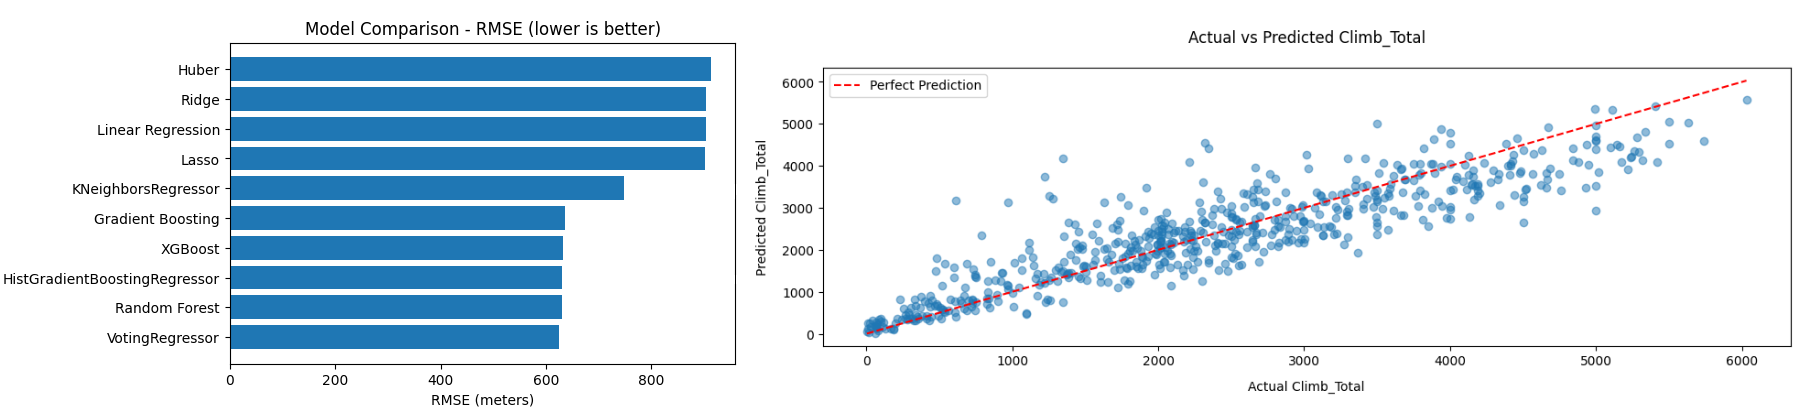
\includegraphics[width=1.0\textwidth]{assets/regressors1.png}
    \caption{Average RMSE for each regressor and Predicted vs Actual values.}
    \label{fig:regressor1}
\end{figure}
\subsubsection{Distribution-based Imputation}
Briefly, the density-based approach clusters races with the \texttt{KMeans} algorithm by using these features: \texttt{length}, \texttt{points}, \texttt{profile} and \texttt{delta}, which demonstrated most effective results. It groups points   : 
\begin{itemize}[noitemsep]
    \item \texttt{length\_category} which can be \texttt{VS} (Very Short), \texttt{S} (Short), \texttt{M} (Medium), \texttt{L} (Long), or \texttt{VL} (Very Long).
    \item \texttt{season\_seg} which can be \texttt{Spring}, \texttt{Summer}, \texttt{Fall}, or \texttt{Winter}.
\end{itemize}
It tests 10 probability distributions - \texttt{dgamma}, \texttt{skewnorm}, \texttt{Student's t}, \texttt{cauchy}, \texttt{laplace}, \texttt{levy}, \texttt{exponnorm}, \texttt{logistic}, \texttt{gennorm}, and \texttt{genextreme} - to best model data scaled to [-1, 1]. We chose these distributions because they can represent both symmetric and asymmetric data patterns around zero and because they offer flexibility in capturing different tail behaviors and skewness while maintaining computational efficiency. 
\\
The distribution selection minimizes the \texttt{total\_score}, calculated as weighted sum of three metrics:
\begin{itemize}[noitemsep]
    \item \textbf{KS statistic} (50\%, is a robust metric): Measures goodness of fit using the Kolmogorov-Smirnov test.
    \item \textbf{Moment score} (30\%, sensible to outliers): Compares mean, standard deviation, skewness, and kurtosis between original data and samples.
    \item \textbf{Density score} (20\%, not always computable): Measures the difference between kernel density estimates of the original and fitted distributions.
\end{itemize}
\begin{figure}[ht]
    \centering
    \begin{minipage}[t]{0.48\textwidth}
        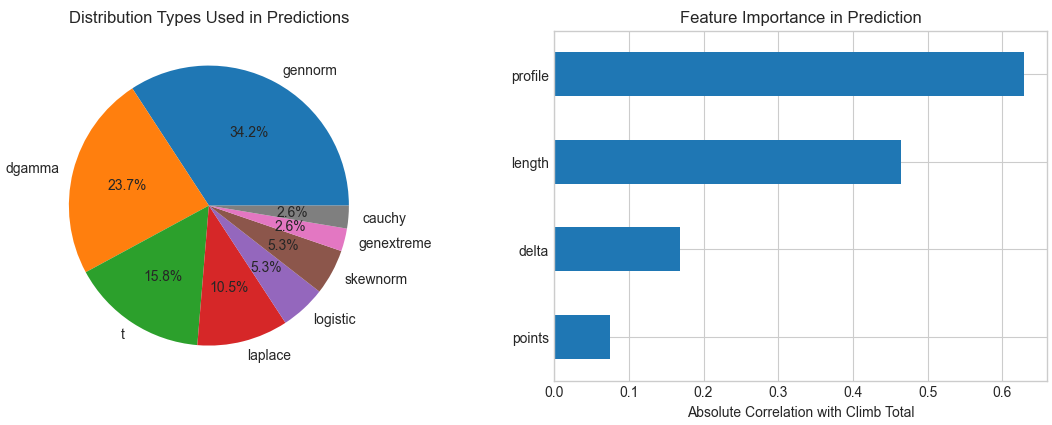
\includegraphics[width=\textwidth]{assets/density_based1.png}
        \caption{Proportion of distributions and features importance for predictions.}
        \label{fig:density-imputation1}
    \end{minipage}%
    \hfill
    \begin{minipage}[t]{0.48\textwidth}
        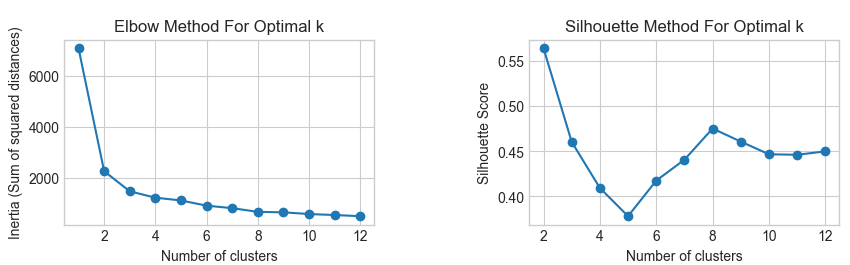
\includegraphics[width=\textwidth]{assets/knn_imputation1.png}
        \caption{Elbow and Silhouette methods for KNNImputer.}
        \label{fig:knn-imputation1}
    \end{minipage}
\end{figure}
\textbf{Results}:
The pie chart in Figure \ref{fig:density-imputation1} shows that the \texttt{gennorm} distribution was selected most frequently, followed by \texttt{dgamma} and \texttt{Student's t}. The feature importance plot indicates that \texttt{profile} and \texttt{length} are the most important features for predicting \texttt{climb\_total}.
\begin{figure}[ht]
    \centering
    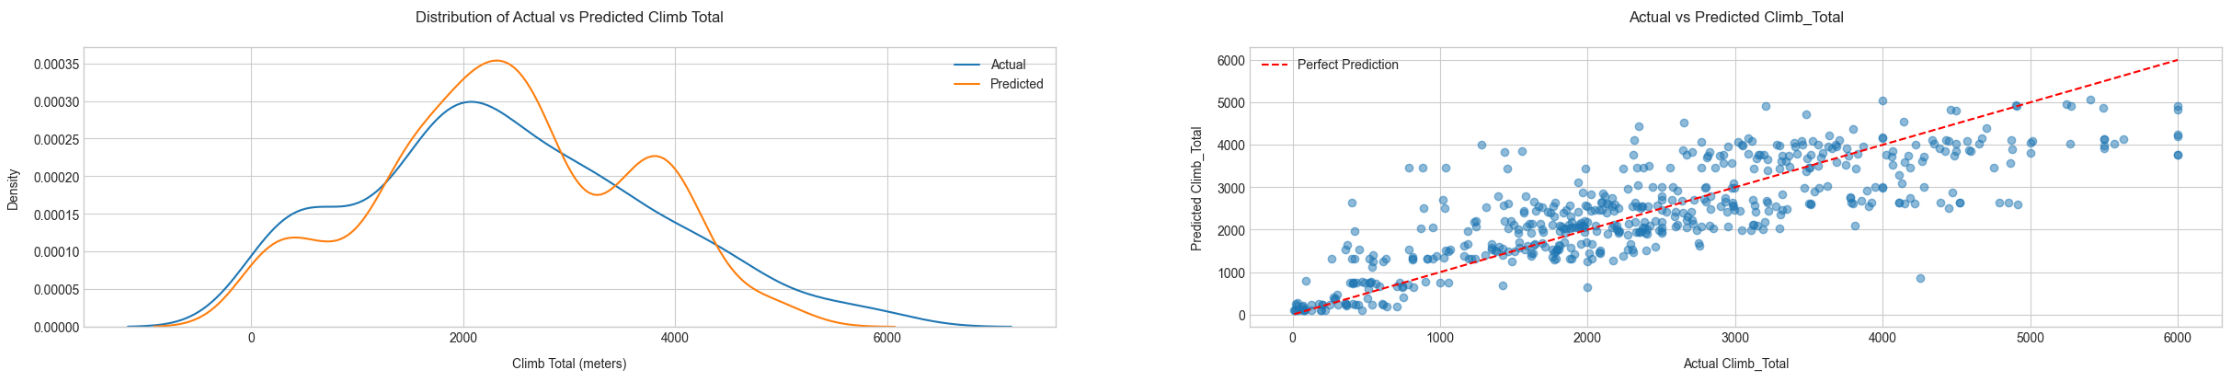
\includegraphics[width=1.0\textwidth]{assets/density_based2.png}
    \caption{Predicted and Actual density plots and scatter plot.}
    \label{fig:density-imputation2}
\end{figure}
The left density plot (Figure \ref{fig:density-imputation2}) shows that an ensemble of densities captures some underlying patterns but not all. The actual values have a wider spread, indicating more variability in real-world data than the model predicts. It overestimates around 2000m, 3800m and underestimates above 4300m, with an average RMSE of around 800m, performing worse than regressors. The density-based approach is reasonably good for predicting \texttt{climb\_total} empty values but is difficult to interpret, stochastic, and requires appropriate distributions picking.
\subsubsection{KNN Imputation}
Our simplest and last approach uses scikit-learn's \texttt{KNNImputer} with n\_neighbors=8 establish by Elbow and Silhouette methods (Figure \ref{fig:knn-imputation1}).
The plots suggest that \textit{k}=8 is a local optimal value, which offers a good balance between cluster tightness and separation.
\\
We used this method for the reason that is simple to implement and computationally efficient and can approximate local patterns. We used these features for the imputation: \texttt{length}, \texttt{points}, \texttt{profile}, \texttt{position}, \texttt{is\_tarmac} and \texttt{cyclist\_age}, since they showed top results.
Its main limitations are:
\begin{itemize}[noitemsep]
    \item Sensitive to the scale of input features
    \item Performance degrades with high-dimensional data
    \item Cannot extrapolate beyond the range of training data
    \item Struggles with complex, non-linear relationships
    \item Might overfit.
\end{itemize}
\textbf{Results}:
The KNN imputer achieved an RMSE of 780m, which worse than the regressors.
\begin{figure}[ht]
    \centering
    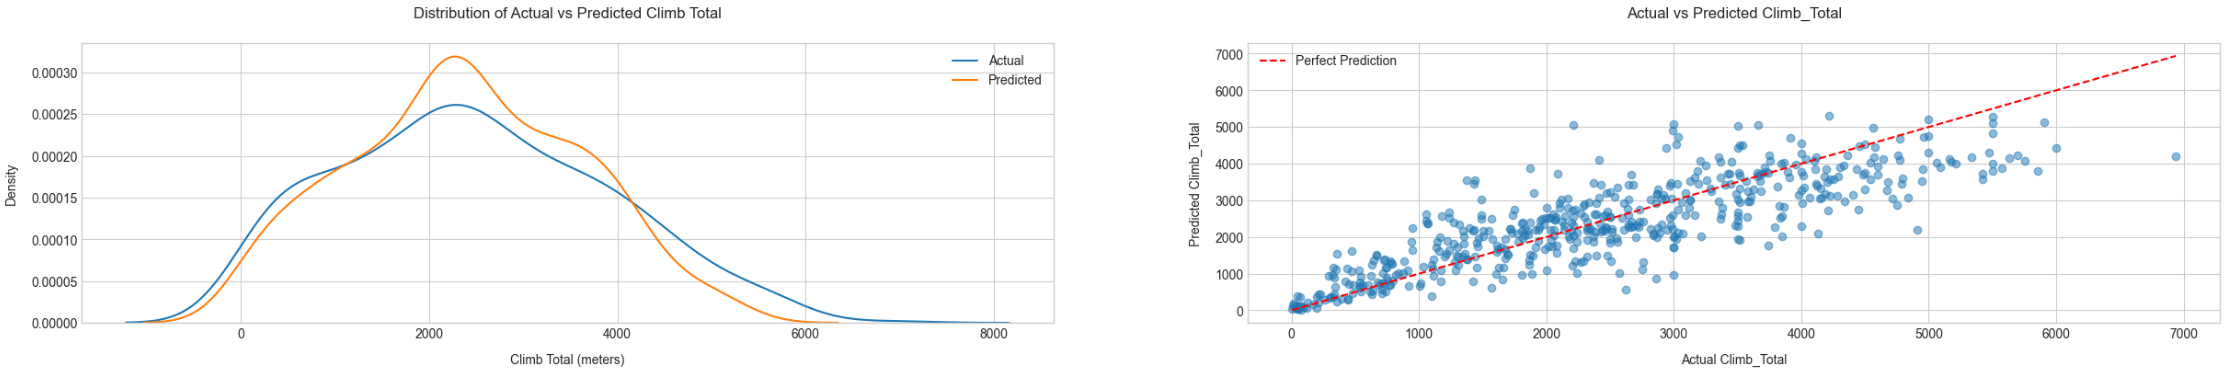
\includegraphics[width=1.0\textwidth]{assets/knn_imputation2.png}
    \caption{Predicted and Actual densities and values.}
    \label{fig:knn-imputation2}
\end{figure}
Looking at the plots (Figure \ref{fig:knn-imputation2}), we can say that the model shows good predictive performance with some tendency to overpredict around 2100m values and underpredict at higher values (above 4000m). The distribution plot (left) shows largely overlapping actual and predicted distributions, though the predicted distribution has a slightly higher peak. The scatter plot (right) demonstrates a strong positive correlation between actual and predicted values, with points clustering around the perfect prediction line but showing increasing variance at higher values.
\subsubsection{Comparative Analysis}

\begin{table}[ht]
\hspace{-0.03\textwidth}
\resizebox{1.06\textwidth}{!}{%
\begin{tabular}{@{}l|l|l|l|l|l|l|l|l|l|l|l@{}}
\toprule
\textbf{Metric} & \rotatebox{0}{VotingRegressor} & \rotatebox{0}{XGBoost} & \rotatebox{0}{Gradient Boosting} & \rotatebox{0}{Random Forest} & \rotatebox{0}{HistGradientBoosting} & \rotatebox{0}{KNeighborsRegressor} & \rotatebox{0}{Lasso} & \rotatebox{0}{Ridge} & \rotatebox{0}{Linear Regression} & \rotatebox{0}{Huber} & \rotatebox{0}{KNN Imputation} \\
\midrule
RMSE (m) & 659.18 & 662.59 & 660.97 & 673.71 & 664.87 & 789.02 & 944.16 & 943.95 & 945.26 & 950.99 & 788.76 \\
R² Score & 0.78 & 0.78 & 0.78 & 0.77 & 0.78 & 0.68 & 0.55 & 0.55 & 0.55 & 0.54 & 0.69 \\
\bottomrule
\end{tabular}%
}
\caption{Comparative analysis of different imputation methods}
\label{tab:imputation-comparison}
\end{table}
Based on the Table \ref{tab:imputation-comparison}, we might say that the VotingRegressor demonstrates superior performance among the tested imputation methods, achieving both the lowest RMSE (659.18m) and highest R² score (0.78). The Density-based and KNN Imputation methods show comparable performance, with KNN having a slightly better R² score (0.69 vs 0.66) despite similar RMSE values. We ought to say that density-based RMSE metric is varying due to the stochastic nature of the method. The value in the table is the average of 10 runs.
The table suggest that ensemble-based regression approaches may be more effective for handling missing values in this particular dataset. Indeed, during other columns imputations, the regressors showed better performance than the other methods. However, the density-based and KNN imputation methods are still valuable alternatives, especially because they obtained better results than the linear regressors.

\subsection{Feature engineering}
Based on our previous analyses, we identified several potential features that could enhance our models. We engineered new features to capture the relationships between existing ones and to provide additional information for our outliers detection and clustering tasks. The new features are:
\begin{enumerate}[noitemsep]
    \item \texttt{pca\_race\_points}: We created it by applying PCA to the \texttt{points} and \texttt{uci\_poi-\\nts} features. We got the best results with 1 component, which explained 95.1\% of the variance. We used it to reduce the dimensionality of the data while preserving the most important information.
    \item \texttt{physical\_score}: We calculated it by combining the \texttt{height}, \texttt{weight}, \\ and \texttt{cyclist\_age} features with the formula: \\
    \verb|(weight / height * 0.6) + (cyclist_age * 0.4)|. \\
    It captures the physical attributes of the cyclists.
    \item \texttt{race\_difficulty}: We produced it by combining the \texttt{length} and \texttt{climb\_total} features with the formula: \\
    \verb|(length * 0.325 + climb_total * 0.525 + is_tarmac * 0.15) / 100|. \\
    It encapsulates the overall race's challenge level.
    \item \texttt{combined\_score\_per\_km}: We determined it by the formula: \\
    \verb|points_per_km * 0.6 + startlist_quality * 0.4|. \\
    This attribute accounts for both the achievements of the cyclists and the quality of the start list.
    \item \texttt{consistency\_score}: We derived it by computing the mean standard deviation of the \texttt{delta}, \texttt{position}, and \texttt{pca\_race\_points} features. This property captures the consistency of the cyclists' performance across races.
    \item \texttt{race\_performance\_score}: As the last engineered feature, we generated it by the formula: \\
    \verb|position_modified * 0.7 + points_per_km * 0.3|. \\
    It provides an overall assessment of the race' performance
\end{enumerate}
We chose these features because they help reduce dimensionality, while preserving the most important information.
\subsection{Outliers detection}
For outliers detection, we applied three distinct algorithms: Local Outlier Factor (LOF), Isolation Forest (IF), and One-Class SVM (OCSVM). We chose these algorithms for their complementary strengths in handling different types of outliers:
\begin{enumerate}[noitemsep]
    \item \textbf{Local Outlier Factor}: We selected LOF for its effectiveness in detecting outliers in datasets with varying densities. It compares the local density of a point to the local densities of its neighbors, making it particularly useful for our dataset where race performances and cyclist attributes can form clusters of different densities.
    
    \item \textbf{Isolation Forest}: We utilized IF for its ability to handle high-dimensional data efficiently and its effectiveness in detecting global outliers.
    
    \item \textbf{One-Class SVM}: We employed OCSVM using GPU acceleration for its robustness in creating a decision boundary that encompasses "normal" data points. This method was particularly useful for identifying outliers in the high-dimensional feature space.
\end{enumerate}
The combination of these three methods provided comprehensive coverage for detecting different types of outliers in our dataset. We categorized the detected outliers into two main groups:
\begin{itemize}[noitemsep]
    \item \textbf{Race Outliers}: Races were classified as outliers if they were flagged by at least one detection methods and had participation numbers above the 50th percentile of all races. E.g. if the same race was consistently identified as an outlier more than 50\% out of all possibilities, we considered it an outlier.

    \item \textbf{Rider Outliers}: Individual cyclists were marked as outliers when they were flagged by at least one detection method and had participated in more than half of races considered as outliers. For example, if a cyclist is listed as participating in more than 50\% of his total races as outliers, we considered him an outlier. 
\end{itemize}

\subsubsection{Motivation}
The ensemble approach of combining LOF, IF, and OCSVM provided robust outlier detection by leveraging each method's strengths while mitigating their individual weaknesses. We opted for these methods rather than alternatives because our dataset contains continues and one categorical features with varying densities, making it more effective to use a combination of methods with different strengths.
These tools provide clear anomaly scores and decision boundaries, making it easier to interpret the results and identify the most significant outliers. In addition, is possible to utilize hyperparameters tuning to improve the performance of the algorithms.
At last, the trio offers complementary perspective on the data, allowing us to capture a wide range of outliers.

\subsubsection{Set up}
Following our experiments, we chose to use these columns in the end: \texttt{nationality}, \texttt{pca\_race\_points}, \texttt{physical\_score}, \texttt{race\_difficulty}, \texttt{combined\_score\_per\_km}, \\ \texttt{consistency\_score} and \texttt{race\_performance\_score} as the most effective for outlier detection. We normalized the numerical features and encoded the categorical data as positive integers.
To evaluate model performance without ground truth outlier labels, we developed a scoring system for outlier detection based on established heuristics described below.
\subsubsection{Tuning and Scoring}
\textbf{Local Outlier Factor}: We randomly selected 30 hyperparameters combinations: \texttt{n\_neighbors} $\sim$ \textit{randint}(15,50), \texttt{contamination} $\sim$ \textit{random.choice}([0.01, 0.05, 0.1, 0.15, 0.2]), \texttt{leaf\_size} $\sim$ \textit{randint}(20-50), \texttt{p} $\sim$ \textit{random.choice}([1, 2]) and \texttt{metric} $\sim$ \textit{random.choice}(['minkowski', 'manhattan', 'euclidean']) possible ones. These values were selected based on our dataset characteristics: \texttt{n\_neighbors} range captures local density variations in our feature space, while contamination levels reflect expected outlier percentages in cycling performance data. The \texttt{leaf\_size} range optimizes the algorithm's performance for our dataset size.
\\
The best LOF model is selected by maximizing a weighted combination of three key components:
\begin{enumerate}[noitemsep]
    \item \textbf{Separation Component (35\%):} it measures how well outliers are distinguished from normal points by comparing their mean scores, normalized by the overall standard deviation. A higher score indicates better separation between outlier and normal populations.
    
    \item \textbf{Density Component (40\%):} it evaluates how different the local density is around outliers compared to the overall dataset density. This component receives the highest weight (0.40) because local density variations are fundamental to LOF's effectiveness.
    
    \item \textbf{Reachability Component (25\%):} it assesses the reachability patterns of outliers versus the overall dataset. It helps identify points that are significantly different from their local neighborhood in terms of distance relationships.
\end{enumerate}
\textbf{Isolation Forest}: We tested 20 configurations with \texttt{n\_estimators} $ \sim $ \textit{randint}(100, 300), \texttt{contamination} $ \sim \mathcal{U}(0.001, 1.0)$, and \texttt{max\_samples} $\sim \mathcal{U}(0.1,0.4)$. The number of trees (\texttt{n\_estimators}) and \texttt{max\_samples} were chosen to balance computational cost and model robustness, while the contamination level was set to reflect the expected proportion of outliers in the dataset.
Our algorithm selection criteria maximizes a composite score based on several key metrics:
\begin{enumerate}[noitemsep]
    \item \textbf{Distribution Metrics (45\%):} considers score STD and skewness to evaluate the spread and symmetry of anomaly scores.    
    \item \textbf{Density Analysis (35\%):} determines the gaps between extreme percentiles and Separation between normal and anomalous points.
    \item \textbf{Control Mechanisms (20\%):} includes outlier penalty and extreme value control limitation mechanism to prevent excessive flagging and manage extreme score distributions.
\end{enumerate}
The final score undergoes logistic transformation and contamination penalty adjustment, ensuring balanced outlier detection. Models with excessive contamination receive exponential penalties, favoring conservative outlier identification.
\\
\textbf{One-Class SVM}: We explored 20 hyperparameters combinations with \texttt{nu} \\ $\sim \mathcal{U}(0.005, 0.015)$, \texttt{gamma} sampled logarithmically in the range $[10^{-5}, 1]$ using $\gamma = e^x$ where $x \sim \mathcal{U}(\ln(10^{-5}), \ln(1))$ to ensure better coverage of different scales, and \texttt{kernel} $\sim$ \textit{random.choice}(['rbf', 'sigmoid']). The \texttt{nu} range was selected to capture the expected proportion of outliers in the dataset, while the \texttt{gamma} range was chosen to optimize the model's performance for our feature space. The kernels were selected based on speed and quality of the results.
The best OCSVM model is chosen based on a weighted combination of multiple components equal to the IF model.
The scores undergo logistic transformation followed by a \texttt{nu} penalty adjustment to ensure balanced outlier detection across the dataset.
\\
The score components of each detector were carefully selected and tested over and over to ensure that they favor models that can detect a wide range of outliers.
\\
\textbf{Results}:
The leftmost plot (LOF) in Figure \ref{fig:outliers_det1} identifies outliers at the periphery and in low-densities regions, mostly. Most outliers are found on the opposite side of the plot.
The middle plot (IF) reveals more global distribution of outliers, regardless of local density. The rightmost plot (OCSVM) demonstrates a more structured decision boundary, with outliers clearly separated in specific regions of the feature space.
\begin{figure}[ht]
    \centering
    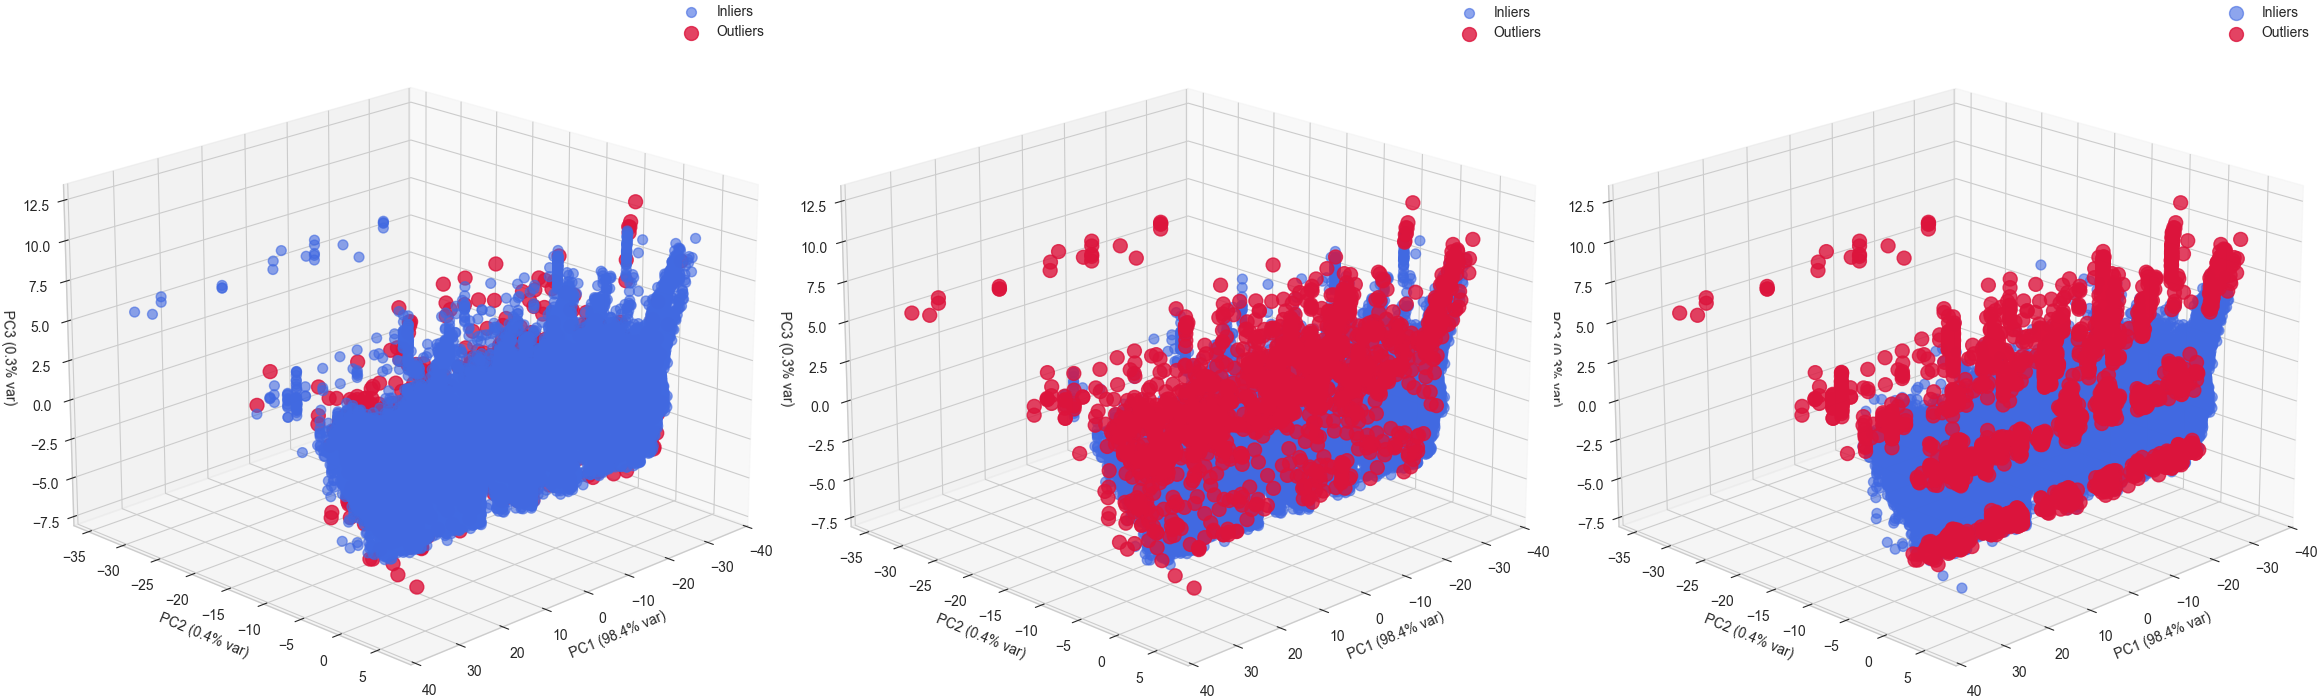
\includegraphics[width=1.0\textwidth]{assets/outliers_det1.png}
    \caption{Outliers detection results for LOF, IF, OCSVM respectively.}
    \label{fig:outliers_det1}
\end{figure}
\subsection{Outliers analysis}
We identified 26 races outliers and 493 cyclists outliers.
The Venn diagram in Figure \ref{fig:outliers_venn} shows the distribution of row outliers across the three detection methods. LOF has detected the most outliers, followed by IF and OCSVM because of its ability to capture local density variations, which cycling performance data often exhibits.
In addition, LOF score metric doesn't penalize outliers as much as IF and OCSVM, which may explain the higher number of detected outliers. IF and OCSVM tend to behave more conservatively.
\begin{figure}[ht]
    \centering
    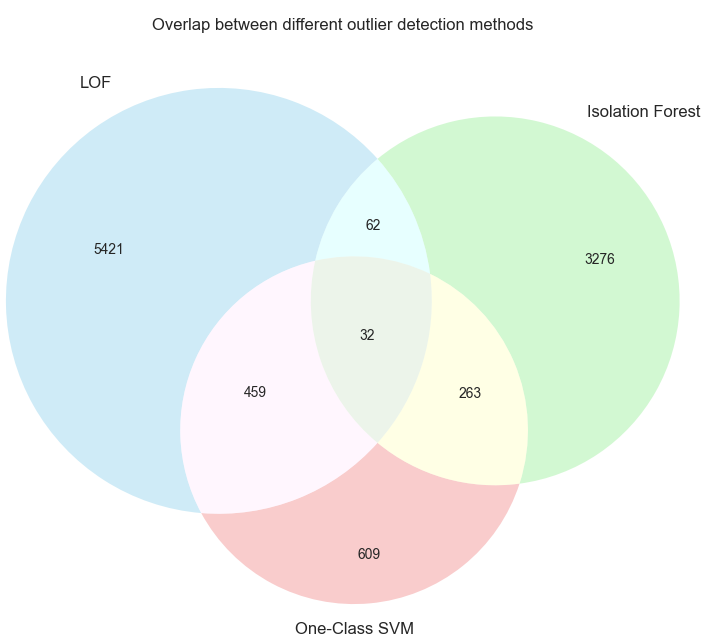
\includegraphics[width=0.4\textwidth]{assets/outliers_venn.png}%
    \caption{Distribution of outliers across \\ detection methods.}%
    \label{fig:outliers_venn}%
\end{figure}%
Figure \ref{fig:feature_importance} displays the feature importance for the outlier detection. We can see that for races (left plot):
\begin{itemize}
    \item \texttt{length} and \texttt{climb\_total} are the most crucial features for detecting outliers, which is expected.
    \item \texttt{profile} and \texttt{startlist\_quality} contribute less to the detection, but they still hold some importance.
\end{itemize}
For cyclists (right plot):
\begin{itemize}
    \item \texttt{cyclist\_age} and \texttt{delta} are fundamental for detecting outliers, which is consistent with our previous analyses.
    \item \texttt{points} and \texttt{uci\_points} have less importance, because they are more volatile metrics that can fluctuate significantly based on short-term performance and race participation, making them less reliable indicators of systematic outliers in cyclist performance patterns.
    \item \texttt{height} and \texttt{weight} surprisingly have very low importance, especially height, which can be explained by the relatively narrow range of these physiological characteristics among professional cyclists. While these metrics influence performance, their variance within the elite cycling population is limited, making them less discriminative for outlier detection compared to performance-based metrics like \texttt{delta} and age-related factors.
\end{itemize}
\begin{figure}[ht]
    \centering
    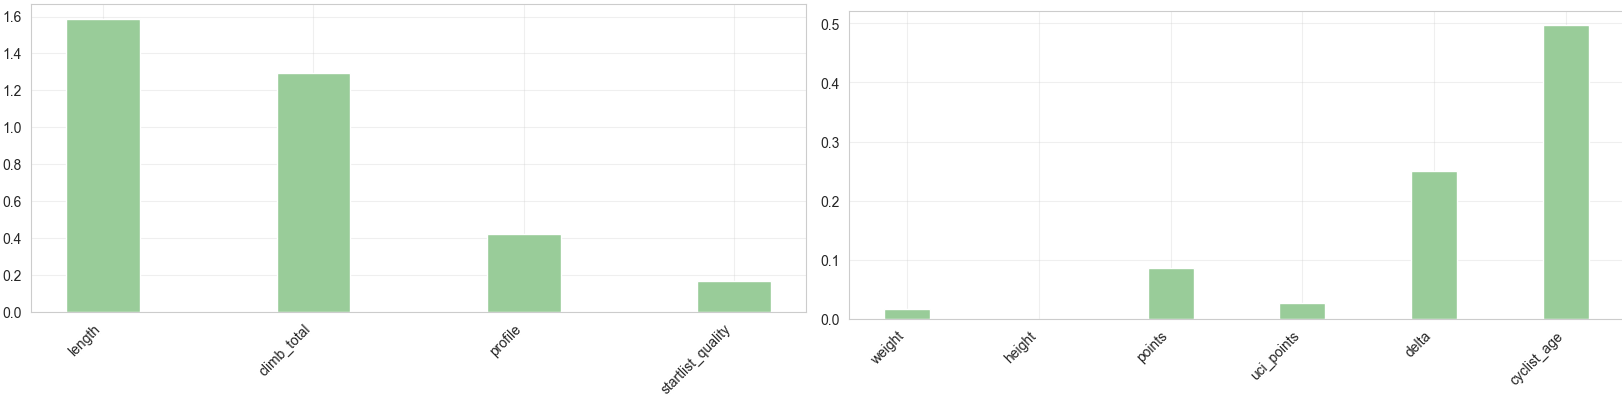
\includegraphics[width=0.7\textwidth]{assets/feature_importance.png}
    \caption{Feature importance for outlier detection.}
    \label{fig:feature_importance}
\end{figure}
\section{Data clustering}

\subsection{K-means}

For this clustering, more tests were done, modifying the value of K and observing how the SSE loss value moved (Figure \ref{fig:SSE-K-means}). Based on the experiments done with K-means, we can observe that as the value of K increases, the SSE loss value decreases. This means that the dataset does not have sufficiently dense regions to be able to define well-defined clusters.
Range tried of K values start from 2 and finish to 20, so in this way is proved a large range of values.

\subsection{DBSCAN clustering}

This section provides information on our implementation and analysis of DBSCAN (Density\-Based Spatial Clustering of Applications with Noise), a clustering algorithm used to identify dense regions in the data and classify points not belonging to any cluster as noise. DBSCAN does not require the number of clusters to be specified in advance. The two critical parameters of DBSCAN, \texttt{eps} (radius of the neighbourhood) and \texttt{min\_samples} (minimum number of points in a neighbourhood to define a cluster), have a significant impact on the quality of clustering. By adjusting these parameters, cluster formation and noise detection can be refined.

\textbf{Data Preprocessing}
The data were scaled using \texttt{StandardScaler}, which standardises features so that they have zero mean and unit variance. Scaling is crucial in DBSCAN, as distances between points are calculated during clustering. For large datasets, scaling helps prevent features with higher number ranges from dominating the clustering process. To avoid computational problems with large datasets, a random sample of 50,000 points was taken to perform the clustering.
Since the dataset does not have a structure that requires a particular metric we used the euclidean distance. For the choice of min-samples since our dataset is 6-dimensional appropriate values can be from 7 to 12. We tried only a few values due to the high computational cost that would have required a more complete choice.

\textbf{Optimization of Parameters}
In the analysis, different combinations of the following parameters were tested. 
\begin{itemize}[noitemsep]
    \item \texttt{min\_samples\_values}: we chose some values between 7 and 12 due to the dimensionality of the dataset.
    
    \item \textbf{eps}: K-distance graphs were generated for ‘k’ values (7, 8, 10, 11, 12) corresponding to potential ‘min\_samples.’ The elbow point consistently suggested ‘eps’ values between 0.9 and 1.2 as optimal for distinguishing clusters.

\end{itemize}
We try different combination, DBSCAN was run and the silhouette score calculated to assess the quality of the clusters. 


\textbf{Results}
The optimal combination of parameters was identified as:
\begin{center}
    \texttt{'eps': 1.2, 'min\_samples': 10, 'Number of clusters': 4, 'Silhouette Score': 0.683, 'Total points': 50,000, 'Total noise points':283}.
\end{center}
The figure \ref{fig:dbscan} shows the resulting clustering visualized with PCA with clusters differentiated by color.

The figure \ref{fig:dbscan} shows 

Finally we calculate the statistical summary for each cluster:
\begin{itemize}[noitemsep]
    \item \texttt{Cluster 0}: encapsulates the average rider population.
    
    \item \textbf{Clusters 2 and 3}: capture specialized subgroups, possibly elite performers requiring further domain analysis.

    \item \texttt{Minimal noise}: suggests robust parameter tuning.

\end{itemize}

\textbf{Conclusions}
DBSCAN effectively clustered dense, high-dimensional data with minimal noise.

Limitations:
\begin{itemize}[noitemsep]
    \item sensitive to parameter variations
    \item Computational cost.
\end{itemize}

\subsection{Hierarchical clustering}

Hierarchical clustering creates clusters progressively, allowing evaluation at different levels of granularity. Using the silhouette score as a measure of clustering quality, we aimed to gain insight into the structure of the dataset and identify the most suitable cluster counting and linking method.

\textbf{Data Preprocessing}
The data was scaled using \texttt{StandardScaler}, which standardizes features to have zero mean and unit variance. This step ensures that features are comparable, since hierarchical clustering relies on distance metrics (e.g., Euclidean distance) that are sensitive to differences in scale.
To address the computational challenges associated with large datasets, a random sample of 50,000 data points was drawn for clustering analysis.

\textbf{Hyperparameter Tuning}
Hierarchical clustering was performed using four linkage methods: \texttt{ward}, \texttt{complete}, \texttt{average}, and \texttt{single}. The dataset was scaled and further reduced to two dimensions using PCA for ease of visualization. The silhouette score was calculated for cluster counts between $t=2$ and $t=14$ to assess the quality of clustering.



\textbf{Results}
\begin{itemize}[noitemsep]
\item The Ward method outperformed other linking methods in forming compact and meaningful clusters, as confirmed by higher silhouette scores and better visual separations. The best silhouette score was $0.637$ at $t=2$. Figure \ref{fig:hc} shows the resulting dendogram, and Figure \ref{fig:hc_pca} shows the resulting clustering visualized with PCA with clusters differentiated by color.
\item The silhouette score peaked at $t=2$ and decreased as more clusters were added, suggesting overfitting or excessive granularity with higher cluster counts.
\item \textbf{Complete and average methods:} These methods demonstrated less consistency and often produced a dominant cluster, especially at lower cluster counts. 
\item \textbf{Single method:} consistently produced a large cluster, resulting in reduced clustering quality and poor silhouette scores.
\end{itemize}

\textbf{Conclusion}
The choice of linkage method significantly affected the clustering results and visual interpretations, highlighting the importance of selecting the most appropriate approach. Hierarchical clustering with the Ward linkage method effectively identified significant patterns in the dataset. It revealed distinct clusters and provided insight into the underlying structure of the dataset. However, some limitations were observed:

\begin{itemize}[noitemsep]
\item \textbf{Scalability:} computational complexity
\item \textbf{Hyperparameter sensitivity:} dependent on hyperparameters
\end{itemize}

\section{Predictive models}

The purpose of this classification analysis is to predict whether a cyclist finished in the top 20 positions of a race, represented as a binary outcome (1 for top 20, 0 for other positions). In order to train the set of models explored during model selection on the data, the dataset on which the data was trained was extracted:

\begin{enumerate}[noitemsep]

    \item The race dataset was taken after the data transformation was processed.

    \item The label label (the target label for training) was calculated by extracting it from the position label: if the position value was >= 20, then label was 0, otherwise label was 1.

    \item The labels: \textbf{\_url}, \textbf{name}, \textbf{date}, \textbf{position}, \textbf{cyclist}, \textbf{delta}, \textbf{race\_year} and \textbf{position} have been removed.

\end{enumerate}

During training, all racing rows from 2022 onwards are considered in the test set, the others in the training set. The input features considered are: \textbf{points}, \textbf{uci\_points}, \textbf{length}, \textbf{climb\_total}, \textbf{profile}, \textbf{startlist\_quality}, \textbf{cyclist\_age} and \textbf{delta}. Note that the classes are unbalanced, in fact both in the training set and in the test set class 1 has a distribution of approximately 14\% and class 0 has a distribution of approximately 86\%.

\subsection{Linear classification}

A linear classifier was used in model selection to see if the problem could be linearly separable. This hypothesis derives from the fact that there may be a hyper-plane that divides the points based on position.  The optimization algorithm was created with the sklearn library, as it allowed the model to be trained very quickly. The training reported metrics with good training values: The training reported metrics with good training values: \textbf{Accuracy}: \textbf{train} value 92.6\%, \textbf{validation} value 92.6\% and \textbf{test} 91.7\%. \textbf{Log-Loss}: \textbf{train} value 0.2230, \textbf{validation} value 0.2250 and \textbf{test} 0.2664. \textbf{AUC}: \textbf{train} value 89.8\%, \textbf{validation} value 89.6\% and \textbf{test} 83.0\%.

\subsubsection{Analysis pattern}

Observing the results obtained by the SHAP tool, it can be concluded that the importance of the most important features are:

\begin{itemize}[noitemsep]
    
    \item  the points feature has a great influence on predicting the class with a positive label, this is explained by the fact that between points and position there is a correlation of -31\%.
    \item  the feature uci\_points has a great influence on predicting the class with a negative label and this justifies why there is a correlation of -16\% between uci\_points and position.
    \item  the delta feature has a little influence on predicting the class with a positive label and this can be confirmed with the correlation between delta and position of -24\%.

\end{itemize}



Overall, the features contribute to recognizing the label 1 little more than 0, and this is explained that model considering more 1 label, because it is in minor distribution.

\subsection{Esembling linear classification}

An example stacking composed of 4 linear classifiers was used: \textbf{LogisticRegression}, \textbf{RidgeClassifier}, \textbf{SGDClassifier} and \textbf{PassiveAggressiveClassifier}, and a \textbf{LogisticRegression meta classifier}. This structure was chosen to see the behavior of this example by putting multiple classifiers to collaborate with each other, and to see if the important features are the same for each classifier. Also for this model the optimization algorithm was created with the sklearn library for very fast training times. The training reported metrics with good training values: \textbf{Accuracy}: \textbf{train} value 92.8\%, \textbf{validation} value 92.8\% and \textbf{test} 91.8\%. \textbf{Log-Loss}: \textbf{train} value 0.2253, \textbf{validation} value 0.2269 and \textbf{test} 0.2576, \textbf{AUC}: \textbf{train} value 89.7\%, \textbf{validation} value 89.5\% and \textbf{test} 84\%.

\subsubsection{Analysis pattern}

The analysis of the patterns captured for this model must be done analyzing classifier by classifier. From the analyzes it can be seen that for the meta classifier, the most important classifier is the \textbf{RidgeClassifier}, with a contribution mainly on the positive class, followed by the \textbf{LogisticRegression} with little more contributions to the positive class, followed by \textbf{PassiveAggressiveClassifier}, with small positive class contribution, and \textbf{SGDClassifier}, with very small contribution more on negative label.

However, LogisticRegression and RidgeClassifier considers same pattern like important, as like as SDGClassifier and PassiveAggressiveClassifier do.

For the \textbf{LogisticRegression} model and \textbf{RidgeClassifier} models:

- \textbf{points} gives a contribution on the positive class, while \textbf{uci\_points} gives an opposite contribution, i.e. on the negative class
- \textbf{delta} gives a little stronger contribution on the positive class

The \textbf{SGDClassifier} and \textbf{PassiveAggressiveClassifier} classifiers have learned the patterns by giving weight to the same features, and the most important ones are:  \textbf{delta}, \textbf{points} and \textbf{uci\_points}, which gives a powerful contribution on the positive class and less powerful on the positive class.

Looking at the general overview, it can be said that the most relevant features, which generally influence the entire ensemble, are: delta, with a correlation with position of -24\%, points, with a correlation with position of -31\% and uci\_points, correlated with position of -16\%. These percentages justify and explain why even in an ensemble of linear classifiers, as in the case of a simple linear classifier, these 3 features are chosen.




\subsection{Neural network}
We selected a classifier based on Neural Network because of its ability to learn complex non-linear patterns in the data. 
The drawback of this model is that it requires computational resources and can be prone to overfitting if not properly regularized. Furthermore, it challenges the interpretability of the model compared to linear models.
The major issue we faced was the class imbalance, which can lead to biased predictions. Indeed, our dataset has a distribution of 15.41\% for class 1 and 84.59\% for class 0.
To address this characteristic, we used the technique called \texttt{SMOTE} (Synthetic Minority Over-sampling Technique) to oversample the minority class and balance the dataset.
Thereafter, 
\subsubsection{Analysis pattern}

\subsection{Support vector machine}
SVM models are well suited for binary classification, especially with high-dimensional feature spaces. These models excel at separating classes by finding a hyperplane that maximizes the margin between them, particularly when the data has a non-linear decision boundary.

\textbf{Feature Scaling}

The data was pre-processed with \texttt{StandardScaler} to standardize all features, which is essential for SVMs. This helps ensure that no single feature dominates the model's decision making, especially when kernel-based methods are applied. SVM is sensitive to the scale of the features, and feature scaling is a critical step when working with SVM.

\textbf{Hyperparameter Selection}

To optimize the SVM model, I ran a \texttt{RandomizedSearchCV} using the following hyperparameters:

\begin{itemize}[noitemsep]
    \item \textbf{C (Regularization)}: Different values of \textbf{C} were explored to tune the strength of regularization. A higher value of C allows the model to better fit the training data, whereas smaller values allow for a smoother decision boundary that could generalize better on unseen data.
    \item \textbf{Gamma}: Different values of \texttt{gamma} were tested, including \texttt{auto} and \texttt{scale} settings and numeric values such as 0.01 and 0.1. Gamma controls the influence of each data point on the decision boundary.
    \item \textbf{Kernel}: \texttt{rbf}, \texttt{poly}, and \texttt{sigmoid} kernels often provide higher predictive power for non-linear problems. However, their computational cost is significantly higher. Given these constraints, the linear kernel was chosen to ensure feasibility without significantly compromising model quality.
\end{itemize}

\textbf{Model Performance}

\texttt{RandomizedSearchCV} was run with 3-level cross-validation to identify optimal hyperparameters based on the F1 score. This allows for efficient tuning while also taking into account model performance on different subsets of data. The following observations summarize the model's performance:

\begin{itemize}[noitemsep]
    \item \textbf{Class 1 Precision and Recall (Top 20 ranked)}: The model performed well for Class 1, with precision and recall around 0.92 and 0.99, respectively, indicating a strong ability to detect the top 20 ranked cyclists.
    \item \textbf{Class 0 Recall (Non-Top 20 Finishers)}: While Class 1 was well predicted, Class 0 had a lower recall of 0.41, suggesting that a significant number of non-top 20 finishers were misclassified as Class 1. This is common in cases with class imbalance, where the model tends to be biased towards the majority class.
    \item \textbf{F1 Score and Accuracy}: Overall accuracy was 92\%, while the weighted F1 score was 0.90. This reflects strong performance, although the disparity in recall highlights a potential area for further model refinement.
    \item \textbf{ROC-AUC Score}: The ROC-AUC score of 0.898 indicates that the model maintains good discriminative ability between the two classes, although efforts could be made to improve the recall for Class 0.
\end{itemize}

\textbf{Limitations}

\begin{itemize}[noitemsep]
    \item \textbf{Class Imbalance}: Class imbalance is evident in the model performance, with significantly higher recall for Class 1 than for Class 0. Methods such as oversampling, undersampling, or weighting could help improve recall for Class 0.
    \item \textbf{Computation Constraints}: The choice of the \textbf{linear kernel} was driven by the high computational cost of alternative kernels that would typically be preferred for problems where the decision boundary is expected to be non-linear.
    \item \textbf{Hyperparameter Space}: While \texttt{RandomizedSearchCV} allowed for exploration, the number of tested hyperparameter combinations was limited (5 combinations). A more exhaustive search (e.g., expanding the range of possible values for \textbf{C} and \textbf{gamma}) could potentially improve results.
\end{itemize}
\subsubsection{Analysis pattern}


\subsection{Decision tree}

The \textbf{Decision Tree Classifier} is a great algorithm for classification, as it can handle both numerical and categorical data and offers a high level of interpretability.

Since the dataset might be unbalanced (with fewer cyclist instances in the top 20), class balancing was handled with \texttt{class\_weight='balanced'}.

\textbf{Model Selection and Hyperparameter Optimization}
We used a grid search to optimize its hyperparameters, considering different values for:
\begin{itemize}[noitemsep]
\item \textbf{criterion}: the function used to measure the quality of a split. Both \texttt{'gini'} and \texttt{'entropy'} were evaluated.
\item \textbf{max\_depth}: a limit on the maximum depth of the tree. We tested values between 5 and 10, as deeper trees can capture more complexity but can also lead to overfitting.
\item \textbf{min\_samples\_split}: The minimum number of samples required to split an internal node, tested between 5 and 15.
\item \textbf{min\_samples\_leaf}: The minimum number of samples required to be in a leaf node, tested between 1 and 5.
\item \textbf{class\_weight}: Handled class imbalance by assigning different weights to classes (tested with \texttt{'balanced'} and \texttt{None}). \end{itemize}

The best performing model produced the following hyperparameters:
\begin{center}
\texttt{'class\_weight': None, 'criterion': 'gini', 'max\_depth': 10, 'min\_samples\_leaf': 1, 'min\_samples\_split': 10}.
\end{center}

\textbf{Performance Evaluation}
After training, the \textbf{accuracy} of the model on the \textbf{training set} was approximately 96.4\%, and the accuracy on the \textbf{test set} was 94.5\%. These values suggest that the model generalizes well to unseen data.

The \textbf{ROC-AUC} score on the test set was 0.89, indicating that the model does a good job of distinguishing between the two classes.

The (weighted) F1 score of 0.94 confirms a good balance between precision and recall in both classes. In particular, while the precision and F1 score for class 1 (the top 20 ranked) are high, the precision for class 0 (not the top 20) is a bit lower, but still significant.

\subsubsection{Analysis model}

To better understand the model's decision-making process, SHAP values were used to interpret the importance of each feature. Two SHAP explanation methods were explored:

\textbf{Interventional explanations}
This approach involves perturbing the data and analyzing how predictions change based on individual features.

\textbf{Distributive Explanations} This approach uses path-dependent perturbation of the tree, assessing the importance of features through the structural properties of the decision tree.

Both explanation techniques yielded insights into which features were most influential. \textbf{Swarm Plots} provide a visual representation of the relative impact of each feature on the model's predictions. Features with the highest importance and variance in their contribution were highlighted.

\subsubsection{Analysis pattern}

To better understand the model's decision-making process, SHAP values were used to interpret the importance of each feature. Two SHAP explanation methods were explored: \textbf{Interventional Explanations} and \textbf{Distributive Explanations}

Both explanation techniques yielded insights into which features were most influential. \textbf{Swarm Plots} provide a visual representation of the relative impact of each feature on the model's predictions. Features with the highest importance and variance in their contribution were highlighted.
The two plots in figures \ref{fig:SHAP_interventional} and \ref{fig:SHAP_distributional}  are similar, this suggests that the model could be quite robust and that it does not have a strong interaction between the features and the predictions. From these graphs we can observe the importance of the features, in particular, 'points' is the feature that impacts the result of the classifier the most, followed by 'delta', while 'cyclist\_age' is the least impactful feature. Therefore significant changes in 'points' and 'delta' will have an important effect on the prediction. Furthermore we can see for each feature how the different values influence the prediction of the class. For example: "points" has a low value in the negative points and a high value in the positive points. This means that an increase in the value of "points" is associated with a greater probability of obtaining a positive result for the target class. For the feature 'length' the opposite is true.

During the initial analysis, we detected a moderate correlation between position and points (-0.31) and a weaker negative correlation with delta (-0.24). The model confirmed these features as the most important for its predictions. Furthermore, the model also identified 'climb\_total' and 'length' as relevant, despite the preliminary correlations with 'position' were very low, almost negligible (-0.04 and -0.01 respectively), suggesting the presence of complex non-linear patterns.



\subsection{Random forest}
The Random Forest Classifier is well-suited for tabular data with complex feature interactions due to its ensemble nature and robustness against overfitting. \\

\textit{RandomizedSearchCV} was selected over \textit{GridSearchCV} for hyperparameter tuning due to its ability to efficiently explore a wide range of hyperparameter settings while reducing computational cost and time.

\textbf{Model Selection and Hyperparameter Optimization}
The following hyperparameters were tuned using \textit{RandomizedSearchCV} with 20 iterations:
\begin{itemize}[noitemsep]
    \item \texttt{n\_estimators}: Number of trees in the forest \{50, 100, 200\}.
    \item \texttt{max\_depth}: Maximum depth of a tree \{4, 6, 8, None\}.
    \item \texttt{max\_features}: Number of features to consider when searching for the best split \{"sqrt", "log2", None\}.
    \item \texttt{min\_samples\_split}: Minimum number of samples required to split an internal node \{2, 10, 20\}.
    \item \texttt{min\_samples\_leaf}: Minimum number of samples required for a leaf node \{1, 5, 10\}.
    \item \texttt{class\_weight}: Handling of class imbalance \{None, "balanced", user-defined weights\}.
\end{itemize}

The model was evaluated using the F1-weighted score to account for imbalanced class distribution, considering both precision and recall.

The best performing model produced the following hyperparameters:
\begin{center}
\texttt{n\_estimators: 100, max\_depth: None, max\_features: None, min\_samples\_split: 2, min\_samples\_leaf: 5, class\_weight: None}.
\end{center}

The optimal hyperparameters from RandomizedSearchCV were used to train the model. The model used: A Random Forest classifier with 
\begin{center}
\texttt{n\_estimators=30} (changed to default for illustration), \texttt{criterion='gini'}, \texttt{max\_features=3}, \texttt{max\_depth=4}, \texttt{min\_samples\_split=2}, \texttt{min\_samples\_leaf=8} and \texttt{bootstrap=True}.
\end{center}

\textbf{Performance Evaluation}
The trained model was evaluated on the test data set, obtaining the values for the metrics shown in the table \ref{tab:metrics}.

\textbf{Accuracy:} The model achieved a high accuracy of 0.95 for the >50 class, suggesting that most predictions for cyclists in the top 20 positions are accurate. The accuracy for the <=50 class was slightly lower at 0.94. \\

\textbf{Recall:} The recall for the >50 class was exceptionally high (0.99), suggesting that almost all cyclists in the top 20 positions were correctly identified. In contrast, recall for the <=50 class was moderate (0.66), meaning that many drivers outside the top 20 were misclassified. \\

\textbf{F1 Score:} The weighted F1 score was 0.95, reflecting a strong balance between precision and recall between classes. \\

\begin{table}[ht]
\centering
\resizebox{.56\textwidth}{!}{%
\begin{tabular}{|c|c|c|}%
\hline%
\textbf{} & \textbf{Predicted <=50} & \textbf{Predicted >50} \\ \hline%
\textbf{True <=50}  & 622 (True Negatives)   & 39 (False Negatives)  \\ \hline%
\textbf{True >50}   & 317 (False Positives)  & 6086 (True Positives) \\ \hline%
\end{tabular}%
}
\caption{Confusion Matrix}
\end{table}


\textbf{Limitations}
\textbf{Class Imbalance}
Despite reasonable performance, class imbalance (939 cases of <=50 vs. 6125 of >50) likely contributed to the disparity in recall and precision between the two classes.

\textbf{Hyperparameter Coverage}
Although RandomizedSearchCV is computationally efficient, it does not guarantee that all possible hyperparameter combinations are explored. Some potentially advantageous configurations may have been overlooked.


\begin{table}[htb]
\centering
\resizebox{\textwidth}{!}{ 
\begin{tabular}{|l|c|c|c|c|c|c|}
\hline
\textbf{Metric} & \textbf{DT (Class 0)} & \textbf{DT (Class 1)} & \textbf{RF (Class 0)} & \textbf{RF (Class 1)} & \textbf{SVM (Class 0)} & \textbf{SVM (Class 1)} \\ \hline
\textbf{Precision}  & 0.95  & 0.91  & 0.96  & 0.93 &  &  \\ \hline
\textbf{Recall}     & 0.99  & 0.67  & 0.99  & 0.70 &  &  \\ \hline
\textbf{F1-Score}   & 0.97  & 0.77  & 0.97  & 0.80 &  &  \\ \hline
\textbf{Support}    & 6139   & 6125  & 6139   & 939 &  &  \\ \hline
\textbf{Accuracy}   & \multicolumn{2}{c|}{0.95} & \multicolumn{2}{c|}{0.95} &  &  \\ \hline
\textbf{Macro avg Precision} & \multicolumn{2}{c|}{0.93} & \multicolumn{2}{c|}{0.95} &  &  \\ \hline
\textbf{Macro avg Recall}    & \multicolumn{2}{c|}{0.83} & \multicolumn{2}{c|}{0.85} &  &  \\ \hline
\textbf{Macro avg F1-Score} & \multicolumn{2}{c|}{0.87} & \multicolumn{2}{c|}{0.89} &  &  \\ \hline
\textbf{Weighted avg Precision} & \multicolumn{2}{c|}{0.95} & \multicolumn{2}{c|}{0.95} &  &  \\ \hline
\textbf{Weighted avg Recall}    & \multicolumn{2}{c|}{0.95} & \multicolumn{2}{c|}{0.95} &  &  \\ \hline
\textbf{Weighted avg F1-Score} & \multicolumn{2}{c|}{0.94} & \multicolumn{2}{c|}{0.95} &  &  \\ \hline
\end{tabular}
}
\caption{Confronto dei risultati di classificazione tra Decision Tree Classifier e Random Forest}
\label{tab:metrics}
\end{table}



\subsubsection{Analysis pattern}
The \textbf{Swarm graphs} obtained for the random forest are very similar to those obtained for the decision tree model, so we can confirm the observations made in Section 5.5.2.




\section{Conclusion}
\cite{test_cite}

\bibliographystyle{plain}
\bibliography{References}

\end{document}